\documentclass{oci}
\usepackage[utf8]{inputenc}
\usepackage{lipsum}
\usepackage{tikz}
\usetikzlibrary{calc}
\usepackage{tabularx}

\title{La doctora Jones y el templo de las mil almas perdidas}

\newcommand{\drawgrid}{%
  \draw[step=1.0,gray,thin] (0,0) grid (3, 2);
  \foreach \i in {1,...,3}{
    \node at (\i-0.5, 2.2) {\scalebox{0.6}{$\i$}};
  }
  \foreach \j in {1,...,2}{
    \node at (-0.2, 3 - \j-0.5) {\scalebox{0.6}{$\j$}};
  }
}
\newcommand{\jones}[2]{%
  \node[fill] (jones) at (#2 - 0.5, 2 - #1 + 0.5) {}
}
\newcommand{\boulder}[2]{%
  \draw[rounded corners, thick, fill=gray] ($(#2 - 0.85, 2.15 - #1)$) rectangle +(.7, .7) {}
}

\newcommand{\arrowsouth}{%
  \draw[->, very thick] ($(jones) + (0, -.25)$) to ($(jones) + (0, -0.8)$)
}
\newcommand{\arrownorth}{%
  \draw[->, very thick] ($(jones) + (0, .25)$) to ($(jones) + (0, .8)$)
}
\newcommand{\arroweast}{%
  \draw[->, very thick] ($(jones) + (.25, 0)$) to ($(jones) + (.8, 0)$)
}
\newcommand{\arrowwest}{%
  \draw[->, very thick] ($(jones) + (-.25, 0)$) to ($(jones) + (-.8, 0)$)
}
\newcommand*{\tabbox}[2][t]{\vspace{-10pt}\parbox[#1][4.3\baselineskip]{20em}{\strut#2\strut}}
\newcolumntype{A}{>{\footnotesize}m{.50\textwidth} }
\newcolumntype{B}{>{\vspace{10pt}}m{.20\textwidth} }


\begin{document}
\begin{problemDescription}
  Luego de años de búsqueda, la doctora Jones ha logrado finalmente encontrar el cáliz de la vida
  eterna dentro del templo de las mil almas perdidas.
  Pero este no es aún el fin de su aventura.
  Tal como lo presagiaban los escritos, al levantar el cáliz de su pedestal, las mil almas que lo
  resguardaban despertaron de su sueño.
  El templo completo se cae a pedazos y la doctora debe escapar rápidamente o quedará atrapada por
  la eternidad.

  El piso del templo es una grilla de $M\times N$.
  Las casillas están numeradas de norte a sur entre 1 y $M$, y de oeste a este entre 1 y $N$.
  La doctora comienza en la casilla (1, 1) y para escapar debe llegar a la casilla $(M, N)$.
  En condiciones normales se podría caminar libremente sobre la grilla, sin embargo, como todo se
  cae a pedazos, en cualquier momento puede caer una roca sobre alguna de las casillas.

  Los eventos ocurren por turnos, habiendo dos fases en cada uno.
  En la primera fase, un número arbitrario de rocas puede caer sobre las casillas.
  Si la doctora se encuentra en una de las casillas donde cae una roca, será aplastada por esta y
  lamentablemente no podrá escapar del templo.
  Una vez que una roca cae sobre una casilla, esta quedará bloqueada y la doctora no podrá moverse
  a ella.
  En la segunda fase, la doctora debe moverse desde la casilla actual a una de las cuatro casillas
  adyacentes en dirección norte, sur, este u oeste (siempre y cuando no haya una roca sobre esta).

  A continuación se muestra un ejemplo para una grilla de tamaño $2\times 3$:
  \begin{center}
  \begin{tabular}{|B|B|A|}
    \hline
      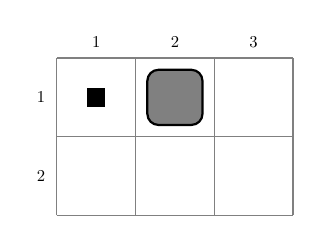
\begin{tikzpicture}
        \drawgrid; \jones{1}{1};
        \boulder{1}{2};
      \end{tikzpicture}
    &
      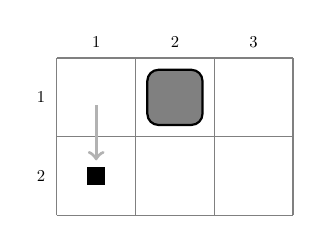
\begin{tikzpicture}
        \drawgrid; \jones{2}{1};
        \draw[->, very thick, color=black!30] ($(jones) + (0, 0.9)$) to ($(jones) + (0, 0.2)$);
        \boulder{1}{2};
      \end{tikzpicture}
    &
    En la primera fase del primer turno una roca cae en la casilla (1, 2) dejándola bloqueada.
    En la segunda fase la doctora se mueve en la única dirección posible quedando en la casilla (2, 1).
    \\
    \hline
      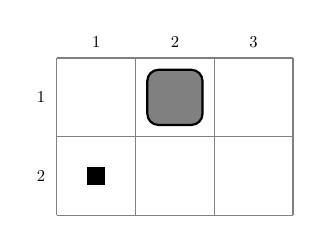
\begin{tikzpicture}
        \drawgrid; \jones{2}{1};
        \boulder{1}{2};
      \end{tikzpicture}
    &
      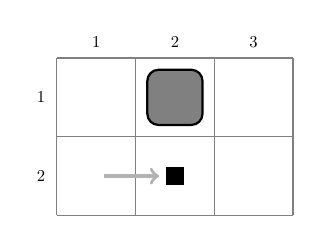
\begin{tikzpicture}
        \drawgrid; \jones{2}{2};
        \draw[->, very thick, color=black!30] ($(jones) + (-0.9, 0)$) to ($(jones) + (-0.2, 0)$);
        \boulder{1}{2};
      \end{tikzpicture}
    &
      En el segundo turno no cae ninguna roca y la doctora se mueve hacia el este quedando en la casilla
      (2, 2).
    \\
    \hline
      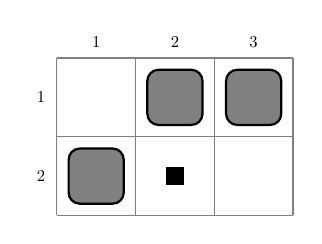
\begin{tikzpicture}
        \drawgrid; \jones{2}{2};
        \boulder{1}{2}; \boulder{2}{1}; \boulder{1}{3};
      \end{tikzpicture}
    &
      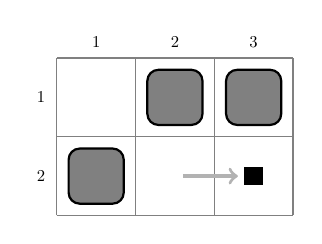
\begin{tikzpicture}
        \drawgrid; \jones{2}{3};
        \draw[->, very thick, color=black!30] ($(jones) + (-0.9, 0)$) to ($(jones) + (-0.2, 0)$);
        \boulder{1}{2}; \boulder{2}{1}; \boulder{1}{3};
      \end{tikzpicture}
    &
      En el turno 3 primero caen dos rocas, una en la casilla (2, 1) y otra en la casilla (1, 3).
      En la segunda fase la doctora se mueve nuevamente hacia el este alcanzando la casilla (2, 3) y
      logrando escapar.
    \\
    \hline
  \end{tabular}
\end{center} 

  En la desesperación, la doctora duda incluso que esta vez le sea posible escapar.
  ?`Puedes ayudarla a saber si podrá escapar o si quedará atrapada para siempre dentro del
  templo?
\end{problemDescription}

\begin{inputDescription}
  La entrada consiste en varias líneas.
  La primera línea contiene dos enteros $M$ y $N$ ($1 \le M \le 1\,000, 2 \le N \le 1\,000$), correspondientes a las
  dimensiones de la grilla.
  La segunda línea contiene un solo entero $K$ ($0 \le K \le M\times N$), correspondiente al número de
  rocas que caerán sobre la grilla.
  Las siguientes $K$ líneas describen la caída de las rocas.
  Cada una contiene tres enteros $t$ ($1 \le t < M\times N$), $i$ ($1 \le i \le M$) y $j$ ($1 \le
  j \le N$), indicando que en la primera fase del $t$-ésimo turno caerá una roca en las coordenadas $(i,
  j)$.
  Se garantiza que nunca caerán rocas sobre las casillas (1, 1) y $(M, N)$.
\end{inputDescription}

\begin{outputDescription}
  La salida debe contener una sola línea con un 1 si existe una forma de que la doctora escape o un 0
  si no.
\end{outputDescription}

\begin{scoreDescription}
  \subtask{20}  % Las bombas no caen al principio o bastaría ver que no haya bombas.
  Se probarán varios casos donde $M = 1$ y sin restricciones adicionales.
  \subtask{30}  % DFS o BFS sirven aquí, el laberinto es estático y flood fill sirve.
  Se probarán varios casos donde todas las bombas caen al comienzo, es decir $t = 1$ para todas las rocas.
  \subtask{50}
  Se probarán varios casos sin restricciones adicionales.
\end{scoreDescription}

\begin{sampleDescription}
  \sampleIO{sample-1}
  \sampleIO{sample-2}
  \sampleIO{sample-3}
\end{sampleDescription}
\end{document}
